\section{Project}
\subsection{Adopted Databases}
According to concept presented in the previous chapter we can make the following considerations:
\begin{enumerate}
\item Because of the performance constraint, a fast back-end is required. Moreover, since the aim is to spread the application worldwide, the database infrastructure should be \textbf{easy to distribute}.
\item \textbf{Pokémon} must store heterogeneous data like URLs, different kinds of bios, float arrays and so on.
\item \textbf{Users} are divided into \textit{normal users} and \textit{admins}. Although the second ones are few, a denormalized approach could be better to handle the fact that these two categories have very different attributes.
\item Rankings are real-time OLAP queries: they need fast aggregation strategies.
\item Favourite \textbf{Pokémon}, \textbf{Friends}, \textbf{Posts} and \textbf{Answers} together form a real Social Network.
\item A \textbf{Team}, in a normalized relational model, could be seen as a relationship table between \textbf{Users} and \textbf{Pokémon}. Anyway, a huge table with a lot of duplicated PokémonID is not scalable due to the requirements of this application. There is a need to find the best way to perform quickly both the retrieving of a \textbf{User}’s team and the ranking of the most used \textbf{Pokémon}, optimizing if possible memory consumption.
\end{enumerate}

The points 1 to 4 guided the choice of a \textbf{Document Database} for handling \textbf{User} and \textbf{Pokémon} data. The \textbf{flexibility}, \textbf{denormalization} and \textbf{performance} of this kind of the database make it the most appropriate one.\medspace \\

The point 5 is best handled by a \textbf{Graph DB}, optimized for networks and different kinds of relationships. Moreover, we realized that the best way to handle a \textbf{Team} is to decompose it in a set of Graph Relationships (USER – OWNS $\rightarrow$ POKEMON).  Indeed, in this way queries mentioned at point 6 are very fast (just counting incoming/outcoming edges, see paragraph 3.3.1), and there are no useless, waste-memory repetitions of User IDs/Pokémon IDs (for a more detailed motivation of this choice see Paragraph 3.4.1). \\
Since each \textbf{User} can have only a \textbf{Team}, \textit{team name} and \textit{points} are stored in the \textbf{User} collection.


\subsection{Document Database}
\subsubsection{Queries Handled}
\textbf{NOTE: the main queries implementation will be presented in the Chapter 4}
\begin{itemize}
	\item Insert a \textbf{User} into the system at registration time
	\item Create a new \textbf{Pokémon} (\textit{admin} only)
	\item Retrieve \textbf{User} information at login time
	\item Retrieve a \textbf{User} by \textit{username}
	\item Retrieve \textbf{Pokémon} information using several filters
	\item Retrieve a \textbf{Pokémon} by \textit{name} when trying to catch it
	\item Modify \textbf{User} settings (\textit{email, password, country})
	\item Update \textbf{Team}’s \textit{name}
	\item Update \textbf{Team}’s \textit{points}
	\item Update \textbf{Pokémon}’s \textit{catch rates} 
	\item Remove a \textbf{User} (\textit{admin} only)
	\item Remove a \textbf{Pokémon} (\textit{admin} only)
	\item \textbf{Analytics}: ranking of best \textbf{Teams} in the world/each \textit{country}/among friends
	\item \textbf{Analytics}: evolution on time of a \textbf{Pokémon} \textit{catch rate}
	\item \textbf{Analytics}: evolution on time of number of logins per day/total \textbf{Users}/logins per day by \textit{country} (admin only)
\end{itemize}
\subsubsection{Entities handled}
Document Database stores information about \textbf{Users} and \textbf{Pokèmons}. \medspace \\ 

In particular it remembers \textbf{User}’s anagraphic and login data, last login, remaining Pokéballs, \textit{team name} and earned \textit{points}; a Boolean field distinguish admin from normal users. Admins have no points nor team or Pokéballs.\\

In a separate collection are stored data about \textbf{Pokémon}: PokédexId (source: PokeAPI), characteristics, one or more types, bio, images URLs, current capture$\_$rate and its last 30 catch$\_$rates stored into an array of floats.\\

The details of the collections are reported in the following paragraph.

\subsubsection{Collections structure}
\begin{figure}[H]
	\centering
	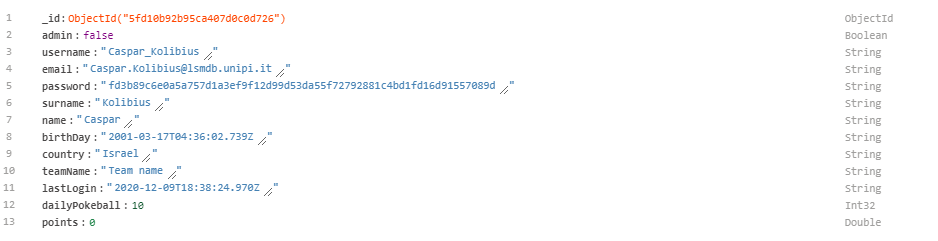
\includegraphics[width=\textwidth]{img/user_collection.png}
	\caption{User Collection}
\end{figure}
Relevant Attributes:
\begin{itemize}
	\item \textit{Admin}: \textbf{true} $\rightarrow$ \textit{admin}, \textbf{false} $\rightarrow$ \textit{normal user}
	\item \textit{Username}: unique mnemonic ID of the user
	\item \textit{Email}: must respect typical e-mail format
	\item \textit{Password}: encrypted version of the user-chosen password
	\item \textit{Last Login}: timestamp of the last time the \textbf{User} logged into the application
	\item \textit{dailyPokeball}: number of daily Pokéballs left. They are up to 10 per day
	\item \textit{points}: worth of his/her \textbf{Team}
\end{itemize}

\begin{figure}[H]
	\centering
	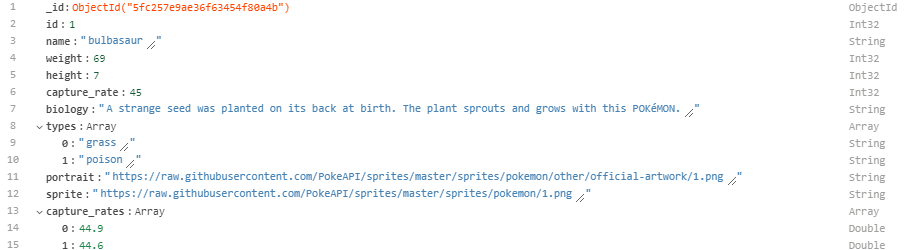
\includegraphics[width=\textwidth]{img/pokemon_collection.png}
	\caption{Pokèmon Collection}
\end{figure}
Relevant Attributes:
\begin{itemize}
	\item \textit{Id}: Pokédex ID (unique)
	\item \textit{Name}: unique mnemonic ID of the \textbf{Pokémon}
	\item \textit{Capture$\_$Rate}: current index of probability to catch the \textbf{Pokémon}
	\item \textit{Portrait/Sprite}: URLs of the graphical representations of this \textbf{Pokémon}
	\item \textit{Capture$\_$Rates}: array of the last 30 values of the capture$\_$rate, one for each of the last 30 days.
\end{itemize}

\subsubsection{Indexes}
All performance tests in this paragraph were made in \textbf{local}.
\subparagraph{Username}
The first field in which we study the possibility of indexing is the \textit{username} one in the \textbf{User} collection. A \textit{username} is a REQUIRED and UNIQUE field of each \textbf{User}, and it is his/her mnemonic id inside the application.
The field \textit{username} is involved in the following queries:
\begin{center}
	\begin{tabular}{|c | c |} 
		\hline
		\textbf{Type} & \textbf{Query} \\ [0.5ex] 
		\hline
		\textbf{W1} & Insert a new \textit{username} at registration time of an arbitrary \textbf{User} \\ 
		\hline
		\textbf{W2} & Remove a \textit{username} when an admin delete’s a \textbf{User} from the system \\
		\hline
		\textbf{R1} & Check uniqueness of a \textit{username} at registration time \\
		\hline
		\textbf{R2} & Check \textbf{User}’s credential at login time \\
		\hline
		\textbf{R3} & Find a \textbf{user} by \textit{username} in order to proceed with a follow/unfollow action \\
		\hline
	\end{tabular}
\end{center}

Assuming that a registered \textbf{User} will play the game for about 100 days before “getting bored”, we can state that the number of logins-per-day will be 100 times the number of registrations-per-day: this means that the queries R1+R2 are submitted 101 times more than query W1.\\
Moreover, we can assert that query W2 will be very rare, while R3 is a popular query among the network structure of the application, say 30 times the number of registered \textbf{Users}: we find out that read operations on this field are about 130 times the number of write operations.
Now consider MongoDb performances with and without using an index on the username field, in a Database populated by 250k users.

\begin{lstlisting}[language=python]
	> db.user.find({username:"eee"},{username:1}).explain("executionStats")
\end{lstlisting}

After submitting the previous command the following results are obtained.

\begin{figure}[H]
	
	\begin{subfigure}{0.5\textwidth}
		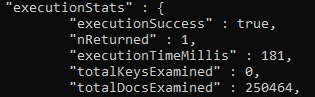
\includegraphics[width=0.9\linewidth]{img/UsernameNoIndex.png} 
		\caption{Results without index}
	\end{subfigure}
	\begin{subfigure}{0.5\textwidth}
		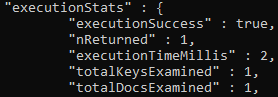
\includegraphics[width=0.9\linewidth]{img/UsernameIndex.png}
		\caption{Results with index}
	\end{subfigure}
\end{figure}

In the picture on the left is reported the output of the query when we do not use an index. Execution time is huge due to the very high number of docs examined. On the contrary, with an index, the same query need an execution time almost 100 times lower, and of course thanks to the index, DBMS only need to examine one document. Moreover the \textit{unique} property permits to eliminate the need of submitting query R1 at each registration.\\
Considering the very high speed-up ratio of the indexing and the high frequency of this kind of queries w.r.t. the write operations (as explained before), \textbf{a UNIQUE INDEX on \textit{username} has been created}.

\subparagraph{Country}
As seen before, starting from the application queries we demonstrate the benefits of an index in the field \textit{country}.

\begin{center}
	\begin{tabular}{| c | c |} 
		\hline
		\textbf{Type} & \textbf{Query} \\ [0.5ex] 
		\hline
		\textbf{W1} & Insert the \textit{country} data at registration time \\ 
		\hline
		\textbf{W2} & Remove all the \textbf{User}’s data if a \textbf{User} is banned by an \textit{admin} \\
		\hline
		\textbf{W3} & Changing of settings after a user changes residence’s \textit{country} \\
		\hline
		\textbf{R1} & Rank all \textbf{Users} by \textit{country} \\
		\hline
		\textbf{R2} & Rank countries with the highest logins-per-day ratios \\
		\hline
	\end{tabular}
\end{center}

Let $x$ be the number of registrations-per-day (W1), w.r.t this number W2 and W3 are very rare operations. Indeed, even though we can expect mischievous behaviours from some user, the number of country changes will never be comparable with $x$.\\
On the other hand, in order to guarantee a read-your-own-write eventual consistency on ranking R1, this query is recomputed every time a user asks to see the ranking itself. Thus, since the gameplay is highly based on rankings, we can estimate that R1 frequency will be about $400x$.\\
Furthermore we have to consider R2. Despite the fact that this query is executed just once per day (so $frequency(R2) \ll x$), it is an asynchronous procedure sensitive to execution time since it needs to lock the entire collection, make it unavailable to users for a while.\\
As seen before, let us compare DBMS performances with and without a country index.

\begin{lstlisting}[language=python]
	> db.user.find({country:"Italy"}).explain("executionStats")
\end{lstlisting}

\begin{figure}[H]
	\begin{subfigure}{0.5\textwidth}
		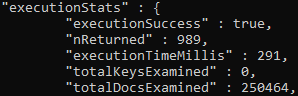
\includegraphics[width=0.9\linewidth]{img/CountryNoIndex.png} 
		\caption{Results without index}
	\end{subfigure}
	\begin{subfigure}{0.5\textwidth}
		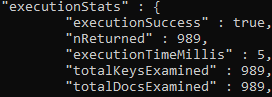
\includegraphics[width=0.9\linewidth]{img/CountryIndex.png}
		\caption{Results with index}
	\end{subfigure}
\end{figure}

Considering again about 250k \textbf{Users}, without an index we need to scan the whole database, which means a medium-high execution time for each request.\\
On the contrary, we have a very high increase of performances introducing and index on \textit{country}: execution time is about 58 times lower and the only documents examined are the ones that must be returned.\\
To summarize, considering the difference in frequency between reads and writes and the high decrease of execution time, \textbf{an index on \textit{country} has been introduced}.

\subparagraph{Pokemon Name}

Queries on \textbf{Pokémon}’s \textit{name}:

\begin{center}
	\begin{tabular}{|c | c |} 
		\hline
		\textbf{Type} & \textbf{Query} \\ [0.5ex] 
		\hline
		\textbf{W1} & Insert a new \textbf{Pokémon} into the Database \\ 
		\hline
		\textbf{W2} & Delete a \textbf{Pokémon} from the Database \\
		\hline
		\textbf{R1} & Search a \textbf{Pokémon} by \textit{name} in the \textit{Pokédex} \\
		\hline
		\textbf{R2} & Browse a \textbf{Pokémon} by \textit{name} in \textit{Catch’Em’All} in order to try to catch it \\
		\hline
		\textbf{R3} & Check \textit{name}’s uniqueness of each \textbf{Pokémon} when added to the database \\
		\hline
	\end{tabular}
\end{center}

Again, W1 and W2 are rare and admin-related operations: this means that this queries will not require a frequent update of the index. On the contrary R1 and especially R2 are very frequent gameplay queries inside the application: we can estimate that R1+R2 frequency will be several orders of magnitude higher than W1+W2 one. \\
R3 instead is a query always required before W1, but it can be managed by DBMS adding a unique property to the index, thus reducing computational cost of the operation itself. \\
In terms of execution time, the final report is the following:  

\begin{lstlisting}[language=python]
	> db.user.pokemon({name: "pikachu"}).explain("executionStats")
\end{lstlisting}
\begin{figure}[H]
	\begin{subfigure}{0.48\textwidth}
		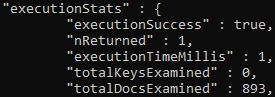
\includegraphics[width=0.9\linewidth]{img/PokemonNameNoIndex.png} 
		\caption{Results without index}
	\end{subfigure}
	\begin{subfigure}{0.48\textwidth}
		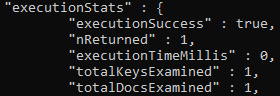
\includegraphics[width=0.9\linewidth]{img/PokemonNameIndex.png}
		\caption{Results with index}
	\end{subfigure}
\end{figure}


Even if we have little changes on execution time due to the limited number of \textbf{Pokémon}, we can see how the index permits to decrease very much the number of examined documents. \\
For the reasons explained before and because of the very high ratio between reads and writes, we consider this little improvement enough relevant for the application purposes. All things considered, \textbf{an index on \textit{pokèmon name} has been introduced}. 

\subsection{Graph Database}
\subsubsection{Queries Handled}
\subparagraph{Users related}
\begingroup
\setlength{\tabcolsep}{10pt} % Default value: 6pt
\renewcommand{\arraystretch}{1.5} % Default
\begin{center}
	\begin{longtable}{|m{0.45\textwidth}| m{0.45\textwidth} |} 
		\hline
		\textbf{Application Queries} & \textbf{Graph Queries} \\ [0.5ex] 
		\hline
		Insert a new \textbf{User} into the system at registration time 		
		& Insert a new USER node into the graph\\ 
		\hline
		Create a \textit{follow} relationship between the current \textbf{User} and the selected \textbf{User}		
		& Add a new FOLLOW edge from the current \textbf{User} Node to the selected \textbf{User} Node \\ 
		\hline
		Retrieve \textit{recommended} \textbf{Users} \textit{by friends}(1)
		& Match all the USER nodes at distance 2 from the given USER node U according to this pattern:
		(U)—FOLLOWS$\rightarrow$(USER f)—FOLLOWS $\rightarrow$(USER recomm.)\\
		\hline
		Retrieve \textit{recommended} \textbf{Users} \textit{by common favourite pokèmons}(2)
		& Match all the USER nodes at distance 2 from the given USER node U according to this pattern:
		(U)—LIKES$\rightarrow$(POKEMON p)$\leftarrow$LIKES—(USER recomm.)\\
		\hline
		Retrieve friend list of a \textbf{User} U
		& Match all the USER nodes linked to the related \textbf{User} Node of U by an outcoming FOLLOWS edge\\
		\hline	
		Retrieve \textbf{User}’s favourite \textbf{Pokémon} 
		& Match all the POKEMON nodes which are linked to the USER node U through a LIKES edge\\
		\hline	
		Remove a \textbf{Pokémon} from the favourite ones
		& Delete a LIKES edge\\
		\hline
		Modify \textbf{User} settings (\textit{country})
		& Modify USER node by changing the country property\\
		\hline	
		Remove a \textbf{User} (\textit{admin} only)
		& Delete a USER node\\
		\hline		
		Remove a \textit{follow} relationship
		& Delete a FOLLOWS edge\\
		\hline
		Analytics: find $\%$ of users that owns a \textbf{Pokémon}
		& Count outcoming HAS edges from the POKEMON node p. 
		Divide the result by the total number of USER nodes\\
		\hline
	\end{longtable}
\end{center}
\endgroup
\subparagraph{Team related}
\begingroup
\setlength{\tabcolsep}{10pt} % Default value: 6pt
\renewcommand{\arraystretch}{1.5} % Default
\begin{center}
	\begin{longtable}{|m{0.45\textwidth}| m{0.45\textwidth} |} 
		\hline
		\textbf{Application Queries} & \textbf{Graph Queries} \\ [0.5ex] 
		\hline
		Retrieve \textbf{Team} composition based on \textbf{User}		
		& Given USER u, retrieve all the POKEMON nodes connected to u through a HAS edge\\ 
		\hline
		Insert a \textbf{Pokémon} into a \textbf{Team}
		& Add a OWNS relationship between a USER node and a POKEMON node\\
		\hline
	\end{longtable}
\end{center}
\endgroup

\subparagraph{Pokemon related}
\begingroup
\setlength{\tabcolsep}{10pt} 
\renewcommand{\arraystretch}{1.5} 
\begin{center}
	\begin{longtable}{|m{0.45\textwidth}| m{0.45\textwidth} |} 
		\hline
		\textbf{Application Queries} & \textbf{Graph Queries} \\ [0.5ex] 
		\hline
		Create a new \textbf{Pokémon} (\textit{admin} only)		
		& Insert a new POKEMON node into the graph\\  
		\hline
		Update \textbf{Pokémon} catch rate
		& Modify USER node by changing the \textit{catch rate} property\\
		\hline
		Remove a \textbf{Pokémon} (\textit{admin} only)
		& Delete a POKEMON node\\
		\hline	
		\textbf{Analytics}: ranking of most popular \textit{Pokémon} in world/each country
		& Count $n_{i} = $ number of HAS incoming edges of POKEMON node $p_{i}$, for each POKEMON node.
		Sort $k$ highest $n_{1}…n_{k}$ and return relative $p_{1}…p_{k}$\\
		\hline
	\end{longtable}
\end{center}
\endgroup

\subparagraph{Post/Answer related}
\begingroup
\setlength{\tabcolsep}{10pt} 
\renewcommand{\arraystretch}{1.5} % Default
\begin{center}
	\begin{longtable}{|m{0.45\textwidth}| m{0.45\textwidth} |} 
		\hline
		\textbf{Application Queries} & \textbf{Graph Queries} \\ [0.5ex] 
		\hline
		Create a new \textbf{Post}		
		& Add a new POST node into the graph\\ 
		\hline
		Create a new \textbf{Answer}	
		& Add a new POST node into the graph\\ 
		\hline	
		Retrieve all the \textbf{Posts} related to a \textbf{Pokémon}
		& Match all the POST nodes which are linked to the POKEMON node P through a TOPIC edge\\
		\hline
		Retrieve all the \textbf{Answers} to a \textbf{Post}
		& Match all the POST nodes which are linked to the POST node P through a TOPIC edge\\
		\hline
		Remove a \textbf{Post} (only \textit{admin} and \textit{post’s creator})
		& Delete a POST node\\
		\hline	
	\end{longtable}
\end{center}
\endgroup


\subsubsection{Entities handled}
The Graph Database stores all the information needed to build the NETWORK INFRASTRUCTURE of the application:
\begin{itemize}
	\item \textbf{User}’s \textit{usernames} and \textit{country}
	\item \textbf{Pokémon}’s name
	\item \textbf{Post}’s \textit{creation date} and \textit{content}
	\item \textbf{HAS relationships} for \textbf{Team} handling, storing also the chosen \textit{slot} for consistency checking
	\item \textbf{LIKES relationships} between a \textbf{User} and a \textbf{Pokémon}, for favourites handling
	\item \textbf{FOLLOWS relationships} between \textbf{Users}
	\item \textbf{TOPIC relationships} between a \textbf{Post} and a \textbf{Pokémon}, in order to see the \textbf{Posts} written about a specific \textbf{Pokémon}
	\item \textbf{TOPIC relationships} also between a \textbf{Post} and another \textbf{Post}, in order to visualize the \textbf{Answers} to a \textbf{Post}  
	\item \textbf{CREATED relationships} between a \textbf{User} and a \textbf{Post} to map the owner of each \textbf{Post}/\textbf{Answers}
\end{itemize}

\subsubsection{Graph structure}
\begin{figure}[H]
	\centering
	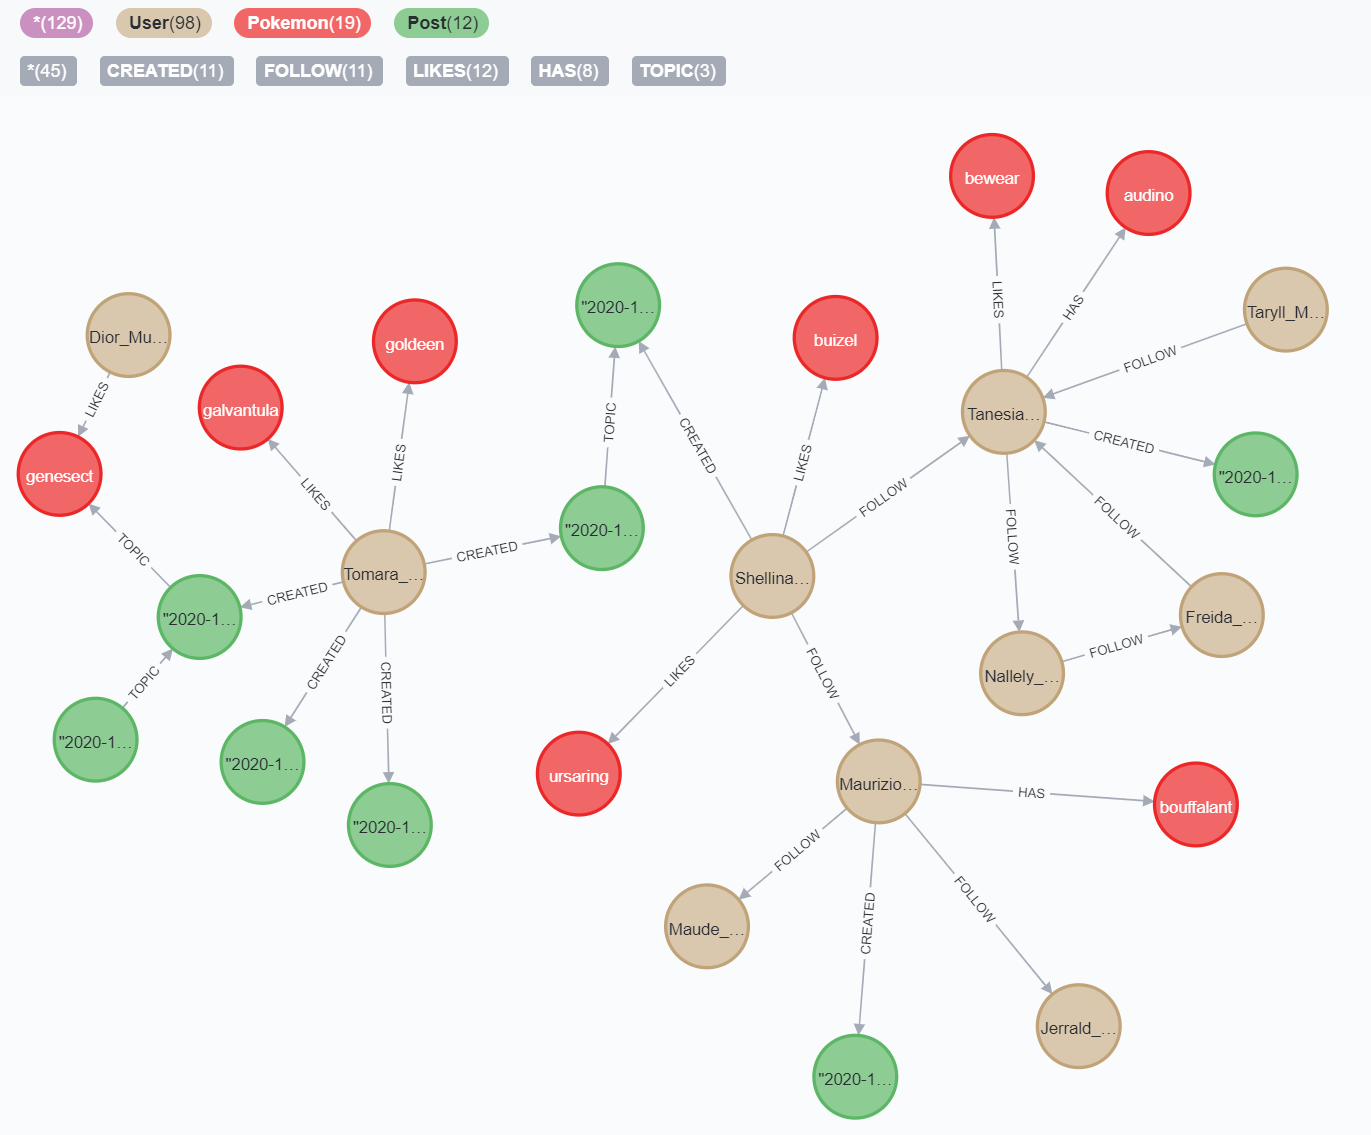
\includegraphics[width=\textwidth]{img/graph_structure2.png}
	\caption{Graph Structure}
\end{figure}

In the previous image a portion of the graph structure is reported. 
\textbf{Pokémon} nodes are red, \textbf{User} ones are brown, green nodes represent \textbf{Posts}.

The properties stored are the following:
\begin{itemize}
	\item USER (node): \textit{country}, \textit{username}
	\item POKEMON (node): \textit{name}, \textit{capture rate},  \textit{sprite}, \textit{type}
	\item POST (node): \textit{content}, \textit{creation date}
	\item FOLLOW (relationship): no properties needed
	\item LIKES (relationship): no properties needed
	\item HAS (relationship): \textit{slot} (integer)
	\item CREATED (relationship): no properties needed
	\item TOPIC (relationship): no properties needed
\end{itemize}


\subsubsection{Indexes}
\subparagraph{Username} As seen in the Indexes Paragraph for MongoDB, the queries that involve the \textit{username} field are the following:
\begin{center}
	\begin{tabular}{|c | c |} 
		\hline
		\textbf{Type} & \textbf{Query} \\ [0.5ex] 
		\hline
		\textbf{W1} & Insertion of a new \textbf{User} in the GraphDB\\ 
		\hline
		\textbf{W2} & Deletion of an existing \textbf{User} in the GraphDB \\
		\hline
		\textbf{R1} & Search of a \textbf{User} \textit{u} by \textit{username} when an answer to a \textit{u}'s P\textbf{ost} is written \\
		\hline
		\textbf{R2} & Search of a \textbf{User} by \textit{username} when a new \textit{follow} request is submitted \\
		\hline
	\end{tabular}
\end{center}
Assuming that the number of new registrations is far more higher that the number of \textbf{Users} deletion, we can state that $|W1| \gg |W2|$. Furthermore, is likely that the number of logins per day are far more than the new registrations at high User number loads, as stated in the Paragraph 2.6 with the load estimation.\\
So, let $x$ be the number of new logins per day, we can say that the number of each read operation will probably be a multiple of $x$, so, at the end, we can state that $|Ri| \gg |W1| \gg |W2|, i = 1,2$. Hence, the application, at the GraphDB side, is \textbf{read intensive} and this statement leads to prove that an usage of an index for this field is good in terms of \textbf{read/write trade-off}.\\
All things considered, from Neo4j Desktop we can compute the following command, which is a simple find by username, in order to get some performance statistics before and after the index addition:
\begin{lstlisting}[language=python]
	neo4j$ explain match (p:User) where p.username = "Grahm_Gschwendtner1989" return p
\end{lstlisting}

\begin{figure}[H]
	\begin{subfigure}{0.5\textwidth}
		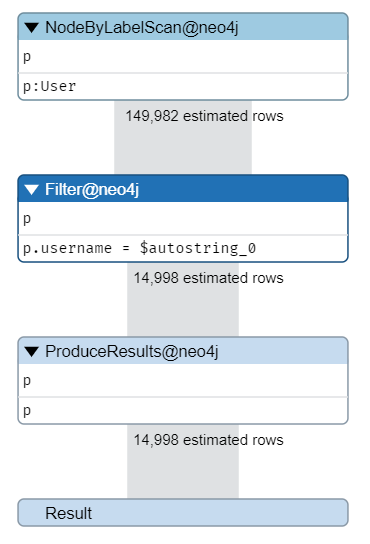
\includegraphics[width=0.9\linewidth]{img/user_without_index_1.png} 
	\end{subfigure}
	\begin{subfigure}{0.5\textwidth}
		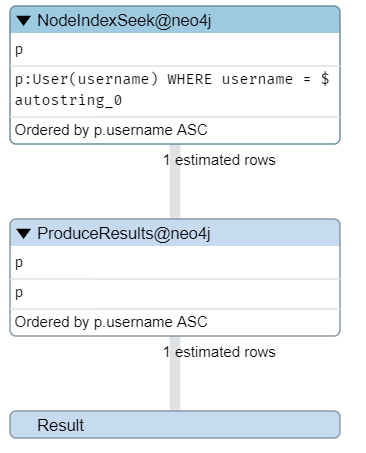
\includegraphics[width=0.9\linewidth]{img/user_with_index_1.png}
	\end{subfigure}
\end{figure}
\begin{figure}[H]
	\begin{subfigure}{0.5\textwidth}
		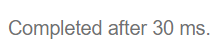
\includegraphics[width=0.9\linewidth]{img/user_without_index_2.png} 
		\caption{Results without index}
	\end{subfigure}
	\begin{subfigure}{0.5\textwidth}
		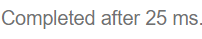
\includegraphics[width=0.9\linewidth]{img/user_with_index_2.png}
		\caption{Results with index}
	\end{subfigure}
\end{figure}

In this case we can notice a \textbf{huge improvement in the number of rows} handled with several order of magnitude and a \textbf{slightly improvement on the timing}. Even if the timing improvement is not huge we have to take into consideration the extreme simplicity of the "find by username" query, which does not show properly the benefits of handling only one row at the beginning of the query computation. All things considered, \textbf{an index on the field \textit{username} has been created.}

\subparagraph{Pokèmon Name}
The queries that involve the \textit{name} field are the following

\begin{center}
	\begin{tabular}{| c | c |} 
		\hline
		\textbf{Type} & \textbf{Query} \\ [0.5ex] 
		\hline
		\textbf{W1} & Insertion of a new \textbf{Pokèmon} in the GraphDB\\ 
		\hline
		\textbf{W2} & Deletion of an existing \textbf{Pokèmon} in the GraphDB \\
		\hline
		\textbf{R1} & Search of a \textbf{Pokèmon} by name in order to catch it \\
		\hline
		\textbf{R2} & Search of a \textbf{Pokèmon} by name in order to create a post on it\\
		\hline
		\textbf{R3} & Search of a \textbf{Pokèmon} by name in order to save it as a favourite \textbf{Pokèmon} \\
		\hline
	\end{tabular}
\end{center}
As said before, the number of addition or deletion of a \textbf{Pokèmon} are extremely rare due to the fact that only the admin could do that. So the writing operation of \textbf{Pokèmon} are done only by the admins where the read operation are done by the normal \textbf{Users}, which number is surely bigger. This consideration is enough to consider the operations on this field as \textbf{read intensive} and is enough to justify the thought of adding an index. In the following figure are presented the query and the relative performance results.
\begin{lstlisting}[language=python]
	neo4j$ explain match (p:Pokemon) where p.name = "pikachu" return p
\end{lstlisting}

\begin{figure}[H]
	\begin{subfigure}{0.5\textwidth}
		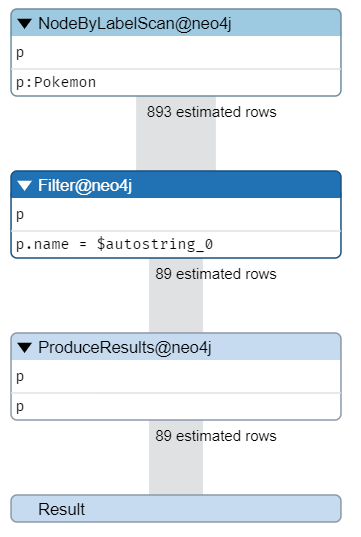
\includegraphics[width=0.9\linewidth]{img/pokemon_without_index_1.png} 
	\end{subfigure}
	\begin{subfigure}{0.5\textwidth}
		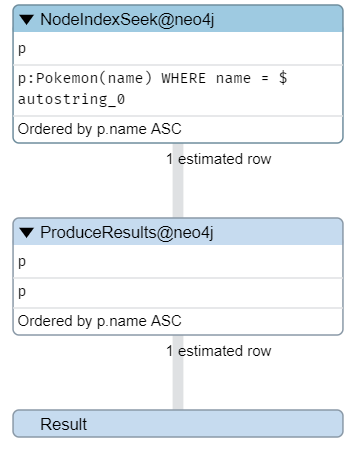
\includegraphics[width=0.9\linewidth]{img/pokemon_with_index_1.png}
	\end{subfigure}
\end{figure}
\begin{figure}[H]
	\begin{subfigure}{0.5\textwidth}
		
\includegraphics[width=0.9\linewidth]{img/pokemon_without_index_2.png} 
		\caption{Results without index}
	\end{subfigure}
	\begin{subfigure}{0.5\textwidth}
		
\includegraphics[width=0.9\linewidth]{img/pokemon_with_index_2.png}
		\caption{Results with index}
	\end{subfigure}
\end{figure}

Even in this case we can see a \textbf{slightly improvement on the timing} performance and an improvement on the rows considered at the beginning of the query computation. The total number of Pokèmon is small with respect to other entities but surely the 3 grade of magnitude of difference for the estimated row should grant a big advantage with bigger and more complicated queries on Neo4j. All things considered, \textbf{an index on the field \textit{pokèmon name} has been added}.
\subparagraph{Post Creation Date}
The queries that involve the \textit{creation date} field are the following

\begin{center}
	\begin{tabular}{| c | c |} 
		\hline
		\textbf{Type} & \textbf{Query} \\ [0.5ex] 
		\hline
		\textbf{W1} & Insertion of a new \textbf{Post} in the GraphDB\\ 
		\hline
		\textbf{W2} & Deletion of an existing \textbf{Post} in the GraphDB \\
		\hline
		\textbf{R1} & Search of a \textbf{Post]} in order to be addressed as a topic of an Answer\\
		\hline
		\textbf{R2} & Search of a \textbf{Post} in order to show every post related to a Pokemon\\
		\hline
	\end{tabular}
\end{center}

In this case we can say $|W1| \gg |W2|$ because only admins and the \textbf{User} who created the it can delete a \textbf{Post}. Then, in general, we can state even that if a \textbf{User} writes, say 1 \textbf{Post} per day, we can surely expect that he isn't the only one who has written a \textbf{Post}. So, in order to write a \textbf{Post} the \textbf{User} will view other \textbf{Posts} of a specific \textbf{Pokemon} (see UML Use Case Diagram for details). We can make the same reasoning even to the replies to a \textbf{Post}, because, in order to make a reply, the viewing action will come first. All things considered, we can assume that all the operation on the \textit{creationDate} of a \textbf{Post} are \textbf{read intensive}. In the following figure are presented the query and the relative performance results.

\begin{lstlisting}[language=python]
	neo4j$ explain match (p:Post) where p.creationDate = "2020-12-15T22:05:32.382000000" return p
\end{lstlisting}

\begin{figure}[H]
	\begin{subfigure}{0.5\textwidth}
		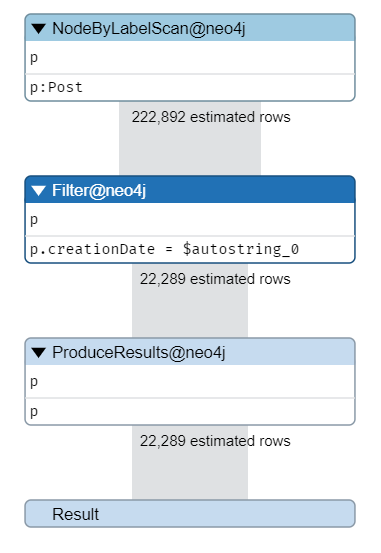
\includegraphics[width=0.9\linewidth]{img/post_without_index_1.png} 
	\end{subfigure}
	\begin{subfigure}{0.5\textwidth}
		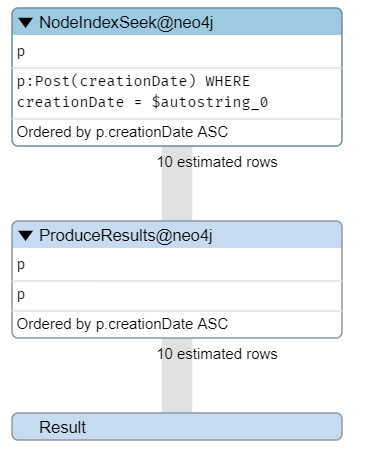
\includegraphics[width=0.9\linewidth]{img/post_with_index_1.png}
	\end{subfigure}
\end{figure}
\begin{figure}[H]
	\begin{subfigure}{0.5\textwidth}
		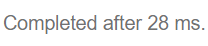
\includegraphics[width=0.9\linewidth]{img/post_without_index_2.png} 
		\caption{Results without index}
	\end{subfigure}
	\begin{subfigure}{0.5\textwidth}
		
\includegraphics[width=0.9\linewidth]{img/post_with_index_2.png}
		\caption{Results with index}
	\end{subfigure}
\end{figure}

We can make the same reasoning made for the \textit{username} field. We can also see that the \textit{creationDate} is not a UNIQUE among all \textbf{Posts} but we can think that filters better than the \textit{content} field. Therefore, \textbf{this field has been chosen specifically for creating an index for the \textbf{Post} entity}.

\subsection{Redundancies and consistency management}
As said in the paragraph relative to non-functional requirements (2.2), performance is an issue for the presented application. Thus we decided, whenever we had to choose from \textbf{fast queries} and reduced memory consumption, to give more importance to the first one, introducing redundancies to minimize pseudo-join operations.
Anyway, this has been done respecting a sort of \textit{“common sense”}, so if we had to choose between spending a lot of memory for a minimum performance improvement or turning down the maniacal hunting of performance to the advantage of a relevant memory saving, we did the second one.  
In the following paragraph are presented the main introduced redundancies and denormalizations, explaining also the implemented consistency mechanism to handle them.

\subsubsection{Team Handling}
In order to maximize response velocity, the \textbf{Team} Entity has been fully denormalized and decomposed. Indeed, as we explained before, a \textbf{Team} is nothing more than a name, and a collection of \textbf{Pokémon} owned by a \textbf{User}. To each \textbf{Team} is associated an amount of \textit{points}, computable starting from the \textbf{Pokémons} composing the \textbf{Team} and their \textit{catch rate}.

Since every \textbf{User} can have only a \textbf{Team}, the \textit{Team Name} property can be directly be stored into the Document Db’s \textbf{User} collection. 
The amount of \textit{points} is not recomputed each time the \textbf{Team} is retrieved but it stored as a redundancy in the user collection until it is changed. \\
The collection of \textbf{Pokémon} is maintained as up to 6 edges between a \textbf{User} node and \textbf{Pokémon} nodes in the \textbf{Graph Database}. This choice is due the fact that:
\begin{itemize}
	\item An array of \textbf{Pokémon} in the user collection was not so good for ranking most used \textbf{Pokémon}
	\item An array of owner \textbf{Users} in the \textbf{Pokémon} collection was bad for retrieving a \textbf{User’s team}.
	\item Considering both the previous arrays was terribly memory-expensive and costly for write accesses. Since the \textbf{Team} is a central game-play write feature, this solution is not suitable.
	\item Considering two arrays in the same fashion as before, but storing IDs instead of plain documents was the worst idea in terms of performance: it would determine a pseudo-join operation for each r/w access.
	\item A \textbf{Team} collection would mean not overcoming the problems given by the relational model. 
	\item Storing everything in a graph, thus repeating \textit{Team Name} and \textit{points} in each relationship was extremely memory-consuming. In the implemented way the retrieving of all the information is still fast since it can be parallelized.
\end{itemize}

\subsubsection{User's Redundancies}
The Document Database’s \textbf{User} collection already stores all the information about each \textbf{User}. Anyway, we decided to replicate some of these attributes in the Graph Database for performance purposes. In particular they are:

\begin{itemize}
	\item \textit{Username}: Despite the fact that DBMSs always provide an identification mechanism not related to the one made by the programmer, we chose to repeat the \textit{username} to quickly retrieve friends’ and post/comment owners’ name. 
	This additional field is not so memory-intensive but can speed-up very much these queries even through the addition of an index, as seen in the Paragraph (3.3.4) 
	\item \textit{Country}. As considered in the Paragraphs (2.6) and (3.2.4), there will be very few \textbf{Users} that will update their settings compared to the ones that will consult rankings. Since the Most used \textbf{Pokémon} by \textit{Country} is a Graph Database query, we decided to introduce this redundancy
\end{itemize}

\subsubsection{Pokemon's Redundancies}
Like for the \textbf{Users}, a Document collection already stores Pokémon information. For similar causes we introduced these redundancies:
\begin{itemize}
	\item \textit{Name, capture rate, sprite, type}: everyone for the same reason that is speeding-up the retrieving of the information needed to capture a \textbf{Pokémon} and it to the \textbf{Team}. In this way adding/removing/finding \textbf{Pokémon} in/from/of a \textbf{Team} is totally handled by the Graph Database, delegating to the Document Database the only task of storing the \textit{team name}. 
	If these speeded-up queries are very frequent (see paragraph 2.6), we can also assert that write accesses to the considered attributes are rare: \textit{name}, \textit{sprite} and \textit{type} are constant values of a \textbf{Pokémon}, and as we will see in the paragraph 3.6, \textit{capture rate} is update only once-per-day.
	Eventually, since \textbf{Pokémon} nodes are very few w.r.t. other nodes, these redundancies are not very memory-expensive
\end{itemize}

\subsubsection{The Analytic Collection}
As said at paragraph 2.1, admin can consult usage statistics in order to evaluate business plans and other possible optimizations. 
To do that, there are two possible approaches:
\begin{itemize}
	\item Computing analytics each time they need them
	\item Storing computed analytics in a separated collection and retrieve them every time they are needed
\end{itemize}

Referring again to our non-functional requirements (par. 2.2), the mechanism that suits best the performance constraint is the second one. 
For this reason, the Document Database hosts also an Analytic collection, structured as follows.
\begin{figure}[H]
	\centering
	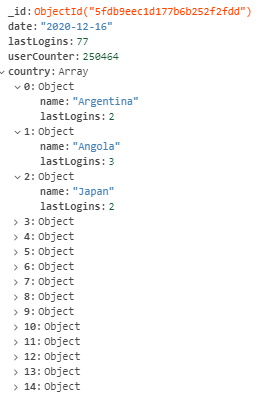
\includegraphics[width= 0.4\textwidth]{img/analytic_collection.png}
	\caption{Analytic Collection}
\end{figure}

This structure is very suitable for the queries presented in the par. 2.1. 
As we will discuss in the par. 3.6, the Analytic collection is updated daily and using a bunch of strategies to minimize the database stress.


\subsection{Database Properties}
\subsubsection{Availability}
A very important non-functional requirement of the application is \textbf{availability}.\\ 
Indeed, \textbf{Users} expect to always have access to the game.
To ensure \textbf{availability}, a cluster of virtual machines has been used, as described in the next paragraph, moreover as reported in paragraphs 3.5.3 and 3.5.4 further mechanism has been projected/implemented in order to guarantee a high level of availability.\\
To ensure it, not only architectural solutions have been exploited, but also software design ones: as described more in deep in the paragraph 3.6, we decided to defer analytics operations, computing aggregate results only once a day (midnight US) instead of every time data is required.\\
This means faster response time of the application during the normal usage, reducing load on the servers. On the other hand, a little overhead in the database is generated at that time, and we have to consider that even if we can estimate a low usage rate in the US at midnight, due to the time zone variation somewhere users might experience some delay. This point is better discussed at the paragraph 3.6.     
\subsubsection{Replicas}
As anticipated in the previous paragraph, the application is provided with replicas support. \\
Replicas are copies of the main server, updated in a deferred way and used not only for backup purposes, but also for taking in charge of some read operations (if configured properly) so that to reduce load on the primary server. \\
The Replicas Architecture used is a Master-Slave fashion, in which only the master can be in charge of write operations.\\
The Replicas Mechanism allows us to ensure a high level of \textbf{availability} of the cluster, overcoming possible server’s crashes/breakdowns. Fault-tolerance and also scalability are guaranteed, together with an accurate design of the eventual consistency, presented in the next paragraph. \\
Even though we achieve a single-server breakdown fault-tolerance, our network is still exposed to a possible down of the link with the cluster.

\subsubsection{Eventual Consistency}
As described before, we preferred guaranteeing low latencies and high availability rather than a strict consistency.\\ 
To be precise, we wanted to achieve a \textbf{read-your-writes consistency} for game players, since they expect that, at the catching/freeing up of a Pokémon, their team and their ranking position is immediately updated taking into account this modifies.
At the same time, we implemented a causal-consistency for the Social Network management: a user usually sees immediately his own posts, but in any way it’s ensured that Posts referring to the same Pokémon will be always in order.
Eventually, for what concerns admins’ analytic data, there is no real consistency warranties that data will be updated: the relative deferred write operation ensures that data has been correctly memorized and journaled, but when a read operation arrive we don’t know if it will pick up new or old data.
\begin{itemize}
	\item The \textbf{read-your-write consistency} is been implemented according to the official documentation of Mongo at https://docs.mongodb.com/manual/ reference/read-concern/\#read-your-own-writes. \\
	So write-concern is majority, read-concern is also majority and read-preference is on the primary when possible (preferred). 
 	\item \textbf{Social Network’s causal consistency} is ensured by the Neo4J framework, that is the specific Graph Database we decided to use(see par. 3.7 for further details)
	\item The \textbf{eventual consistency for usage analytic data} is structured this way: On write operations, the control is returned to the application if the majority of the servers in the cluster have acknowledged it and only after the operation has been correctly journaled. As described by MongoDb documentation, this is enough to guarantee that the operation cannot be lost. Other servers’ data will be eventually consistent, anyway reads are performed in just one of the secondaries, regardless the received data is updated, so that the aggregation operations will not deteriorate server’s performance. Since we have no control on which secondary server will be in charge of each read operation, we cannot ensure any kind of consistency, in fact:

	\begin{itemize}
		\item \textbf{Read} and \textbf{writes} are made from different actors, so is \textit{meaningless} talking about \textbf{read-your-writes consistency}
		\item Since there are \textit{no sessions}, it’s pointless considering a sort of \textbf{session-consistency}
		\item We cannot ensure \textbf{monotonic-read-consistency}: since we don’t know the secondary server that will be in charge of each read operation, it can happen that, given two reads $r_{i}—HB \rightarrow r_{i+1}, r_{i}$ reads from an updated server while $r_{i+1}$ doesn’t.
		\item Theoretically we have no \textbf{monotonic-write-consistency} since the connection with the servers crosses Internet, so we cannot know if an older write request will be received after a newer one. \\
		From a practical point of view we are sure that this kind of consistency will be always guaranteed, due the fact that 2 consecutive writes come 24 hours one from the other
		\item There are no cause-effect relationship in this kind of data, so no eventual consistency		
	\end{itemize}
\end{itemize}

Anyway, there is no need to achieve a strict consistency on admin analytic data, so we preferred to guarantee a lower level of latency, accepting temporary inconsistencies on this kind of data.
\subsubsection{Sharding}
\textbf{N.B.} Despite the fact that we projected here a Sharding mechanism, this is not been implemented in the database cluster. \medskip \\
\textit{Sharding} consists on partitioning data according to a specific policy. Data can be retrieved in the right server/cluster/partition using a Sharding Key.\\
A good Sharding algorithm is the one that permits to retrieve quickly data, but also to partition it homogeneously.\\
In our application we chose to design a \textbf{Geographical Sharding}: each partition is in charge of data generated by \textbf{Users} coming from a specific bunch of \textit{countries}. This kind of division is able to guarantee both the properties discussed before.
\begin{itemize}
	\item It’s \textbf{easy-to-retrieve} because the Sharding Key is a pure key, thus it does not need any computation. As we will see in the chapter 4, it’s convenient to keep in memory (caching) data of the \textbf{User} currently logged: this means that the calculation of the Sharding Key is no more than a simple read access in the main memory
	\item It’s also \textbf{homogenous} if we plan accurately how to partition countries among servers/clusters. Indeed it’s not realistic to assert equal usage distribution on every country, but could either not being enough partitioning according to continents/areas.\\
	Against this problem the most useful tool provided by the application is the usage analytic collection: in this way admins are always updated on the amount of load generated by each \textit{country}, and so they can plan wisely how and where to dispose servers/clusters.\\
	In this way a further optimization could be applied to the application: whereas a cluster is in charge of a particular area, analytic aggregations could be performed  at local midnight instead of at 00:00:00 U.S.\\
	(eg. Let us suppose that, starting from the analytic data provided, admins decided to put a new server on the north of Italy to serve Italy, Switzerland and Austria. We could change the application so that the daemon thread that computes analytic data will go in execution at 00:00:00 Central Europe instead of 00:00:00 U.S.)
\end{itemize}
\subsubsection{Pros and Drawbacks}
Starting from the characteristics of the database infrastructure described in this paragraph, we can state the following considerations:
\begin{enumerate}
	\item The followed project approach prefers in \textbf{general performance} over storage saving. Thus, to guarantee a good game experience with over 5M of users a discrete storage capability is required.
	\item \textbf{Availability} is ensured by always-on servers and use of replicas. However there could be little delays when analytics are written. 
	\item There is \textbf{no strict consistency} among different servers, for no service. For our purposes, \textbf{eventual consistencies} are been finely designed depending on the specific task. They can be consulted at the paragraph 3.5.3.
	\item The \textbf{architecture is the master-slave one}: this means that master can be a \textit{single point of failure}. Although, DBs adopted are capable of performing an \textit{election} in case of primary’s fault, in this case the system will be still capable of working but every NON-JOURNALED write will be lost.  
	\item In spite the fact that this is a performance-centred project, we decide to \textbf{repeat rankings computing} each time a read request arrives. Surely this is not the fastest approach, but we thought that providing a user each time the most updated ranking possible was the best way to encourage him/her to play and try to climb the charts.
\end{enumerate}

\subsection{Client, Server and Daemon Thread}
The \textit{architecture} of our application involves the presence of clients, that will be the \textbf{Users}’ devices, and of some servers that will run in one ore more clusters of machines and that will handle all the data according to the instructions given by clients.\\
The applicative code runs entirely on the clients: every interaction with the GUI is handled locally and may trigger a send of a request to the database.\\
In order to minimize servers’ computational load, they do not execute applicative code, but they only are in charge of providing answers to queries.\\
This means that the application has not been designed as independent from the database infrastructure, but as we will discuss in chapter 4 an accurate information hiding mechanism prevents strong dependencies on the back-end implementation.\\
Apart from the usage analytics (and image download/caching), the applicative code is synchronized with query responses: it stops waiting for an answer from the database. \medskip \\
As already cited before, an analytic function is performed in a deferred fashion every day at 00:00:00, and it is in charge of computing usage statistics rather than updating all \textbf{Pokémon}’s catch rates. \\
Thus, a \textbf{daemon thread} is required: it wakes up at 00:00:00, aggregates data as described in par. 2.5, updates the \textbf{Analytics} collection on the Document Database and eventually sleeps for 24 hours.\\
This operation cannot be performed by normal clients, since it can be computed only once for everyone and it would require a \textbf{User} to have his own device always on; anyway we wanted not to make it be performed by servers, both to reduce their computational efforts and because we cannot take for granted physical access to the server’s file system. \medskip \\

For those reasons we decide to introduce an additional “special” client in which to host the \textbf{daemon thread}. This client must be always-on, does not need high computational power nor a large amount of memory and runs his own piece of applicative code.\\
To simulate its presence, we implemented its methods/classes in a \textbf{separated module} of the application, so that we have no coupling at all between normal clients and this one. \\
\textbf{N.B.} : admin’s devices are normal clients!\\
In the following picture a schema of the application architecture is reported.

\begin{figure}[H]
	\centering
	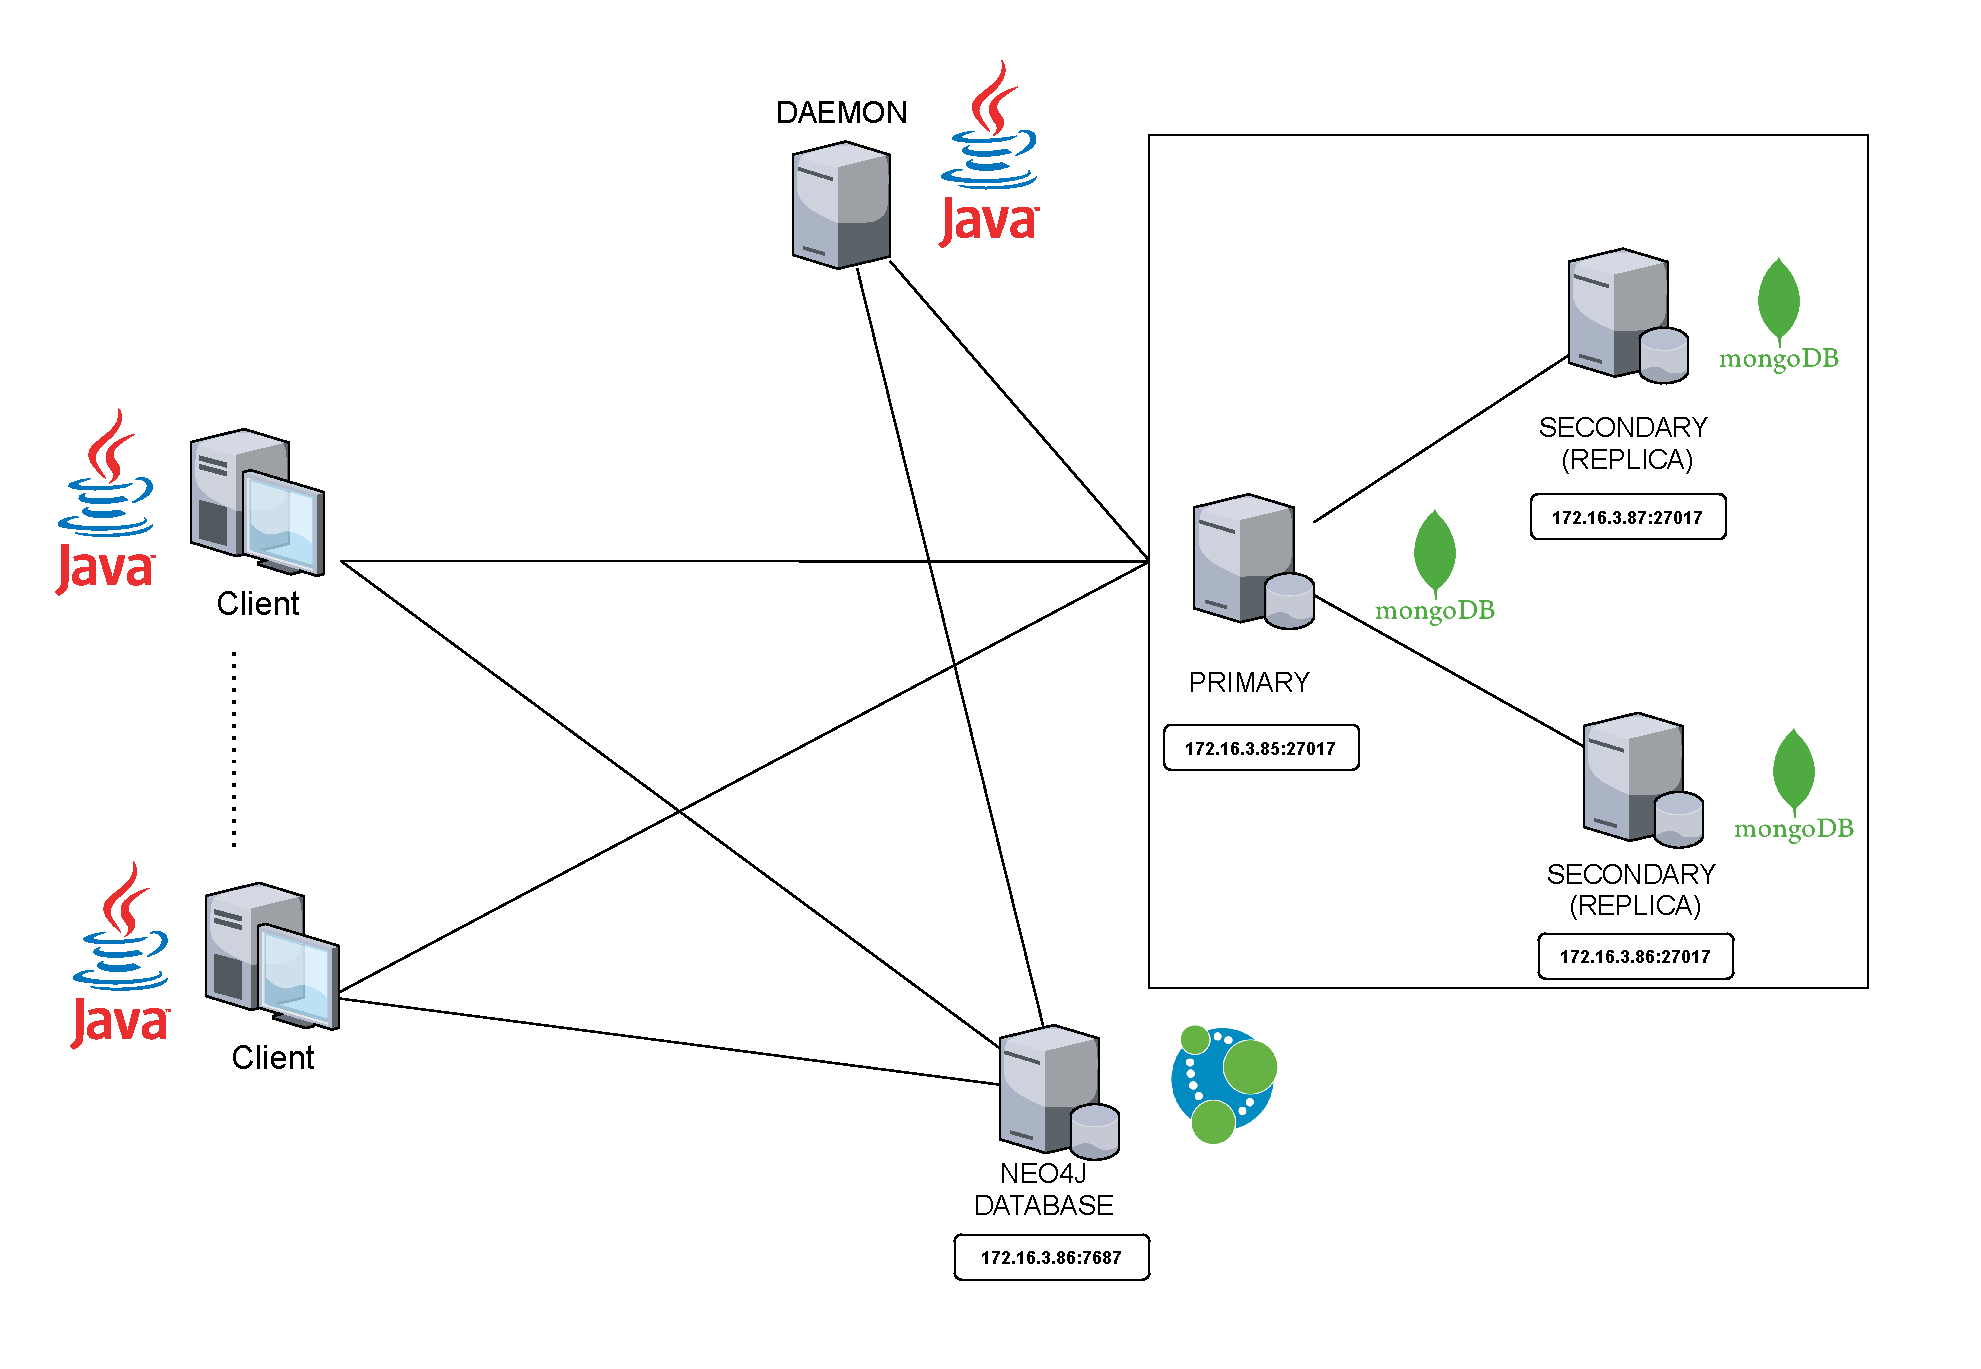
\includegraphics[width=\textwidth]{img/schema2.pdf}
	\caption{Service Architecture}
\end{figure}


\subsection{Technologies and Frameworks}
The most important technologies and framework we chose to build up our project are discussed here. For a more accurate report of these refer to chapter 4.
\begin{itemize}
\item As Document Database we chose is \textbf{MongoDB}: this framework is very easy-to-use, is suitable for large data collections and supports indexing, clustering, replica sets and Sharding. DMBS is optimized for analytics, and the query language is very well integrated with the most famous programming languages.
\item The Graph Database selected is \textbf{Neo4J}, an intuitive and powerful framework, supports indexing, clustering and replicas. Neo4j provides a very expressive query language and some fundamental ensured properties, like Safety (fault-tolerance), Scaling (through Replicas) and \textbf{Causal Consistency}.
\item The main programming language used is \textbf{Java 8}. It provides \textbf{JavaFX support} for GUI design, drivers for the communication with databases and it is compatible with all the main available frameworks/plugins
\item \textbf{Maven} as build and dependency manager, it is been used to organize the code, support pre-build tests, import quickly dependencies and dividing the project into the two modules as explained in the previous chapter
\item \textbf{Junit} for testing classes/methods and for fast bug discovering/recovering    
\end{itemize}
